\begin{chapter}{Results and Discussion}
    I have gone through various studies, most of them are translation and not transliterations. So it's not fair to call my study better than them. But managed to use a data size some what comparable to one of the detailed study.

\par Following Table represents the dataset used in \cite{statIndic}

\begin{table}[h]
\centering
\begin{tabular}{|c|c|}
\hline
Language & Sentences (in millions) \\
\hline
Assamese (AS) & 0.14 \\
Malayalam (ML) & 5.85 \\
Bengali (BN) & 8.52 \\
Marathi (MR) & 3.32 \\
Gujarati (GU) & 3.05 \\
Kannada (KN) & 4.07 \\
Hindi (HI) & 8.56 \\
Oriya (OR) & 1.00 \\
Punjabi (PA) & 2.42 \\
Telugu (TE) & 4.82 \\
Sindhi (SD) & 1.95 \\
Sinhala (SI) & 8.68 \\
Nepali (NE) & 3.35 \\
Tamil (TA) & 5.16 \\
Urdu (UR) & 8.95 \\
\hline
\end{tabular}
\caption{Parallel corpus statistics for English to Indic languages}
\label{tab:parallel-corpus}
\end{table}

In our studies, we have used a 3MB file from the OPUS Data website \cite{opusData} and converted it into Manglish text as a reverse translation. This process itself is time-consuming. After pre-processing was done model was built.

In an SMT-based study in \cite{statIndic}, they got a BLEU Score between 0.46 to 13.09 and 0.49 to 15.41 respectively by checking various settings.

In our study, we obtained a BLEU score of 49.52. I don't claim it as n-times better than the other study \cite{statIndic}, as those are translations. But, I do think transliteration models might perform well on transformer models.

Here is sample sample outputs I found during the evaluation.

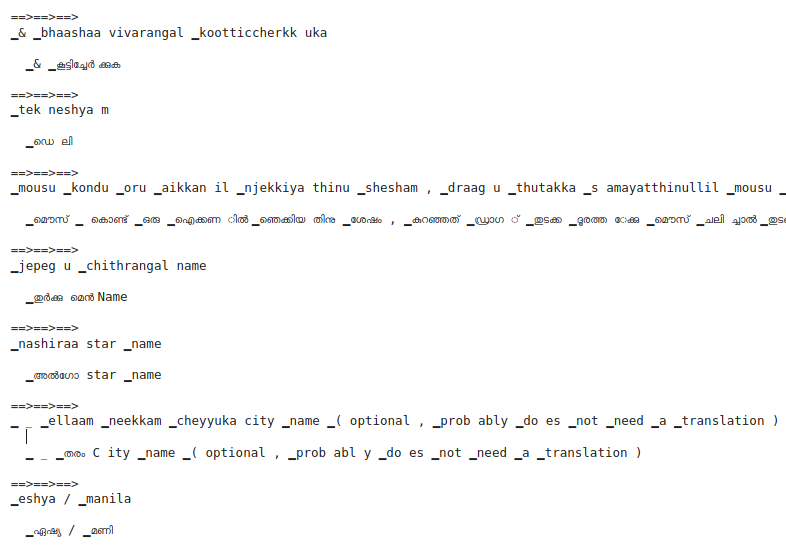
\includegraphics[width=\linewidth]{Images/transliteration_output.png}

\end{chapter}